\section{现阶段研究基础}

\subsection{问题定义}
\begin{frame}{\insertsection}
	1)野外取样
	\begin{center}
		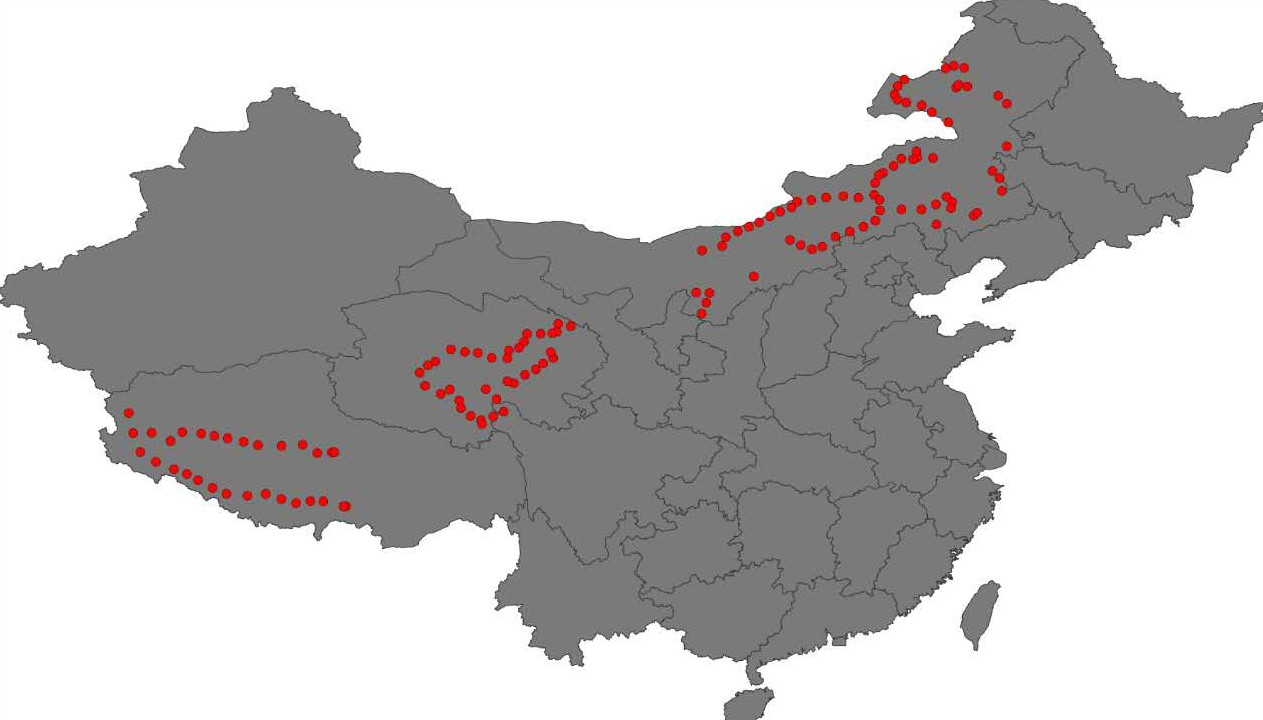
\includegraphics[width = 0.9\textwidth]{./pic/研究方法.jpg}
	\end{center}
\end{frame}
\begin{frame}{\insertsection}{\insertsubsection}	
	2)室内实验:
	\begin{itemize}
		\item 植物样品:已完成西藏、青海两条样带的植物样品采集和分种生物量;
		\item 土壤理化性质:已完成西藏线各理化指标的测定;
		\item DNA提取:已完成西藏、青海、内蒙三条样带的土壤微生物DNA提取工作;
		\item PCR:已完成西藏和青海样带的细菌和真菌的PCR、凝胶回收;
		高通量测序:已完成西藏和青海样带细菌的测序;
	\end{itemize}	
\end{frame}
\subsection{解决思路}
\begin{frame}{\insertsection}{\insertsubsection}
\end{frame}

\begin{frame}{\insertsection}{\insertsubsection}


\end{frame}
